\section{Interessengruppen}

\section{Onion-Diagramm}
\begin{center}
  \begin{figure}[ht]
    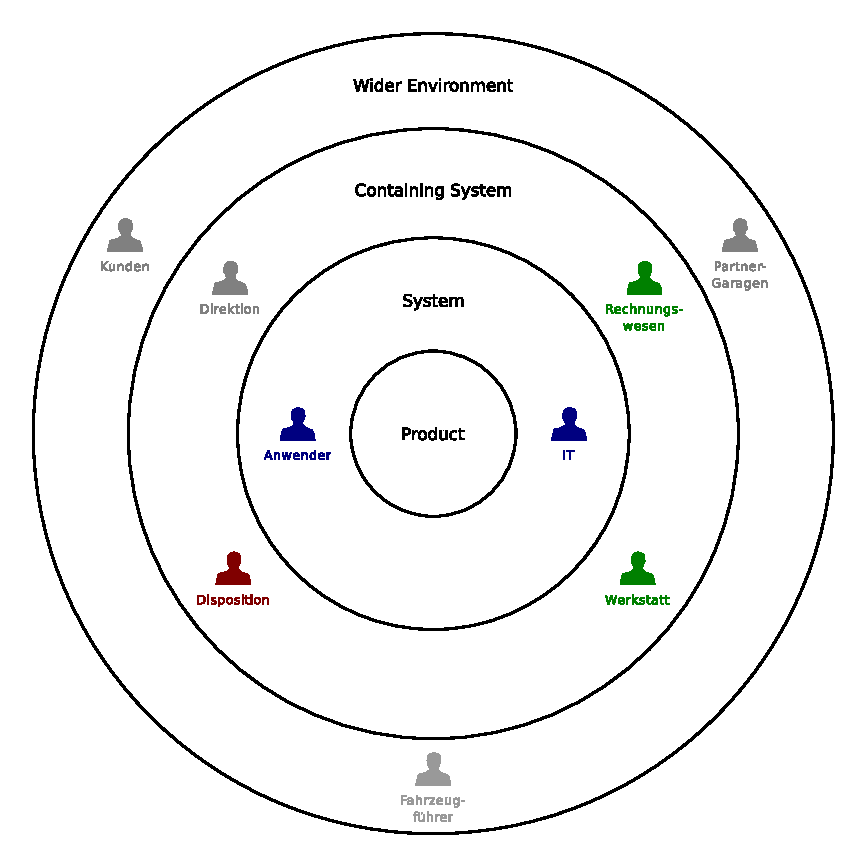
\includegraphics{graphics/onion.pdf}
    \caption{Onion-Diagramm der Nutz AG Steakholders}
    \label{fig:awesome_image}
  \end{figure}
\end{center}

\subsection{Anwender}
Die Anwender sind für die Verwaltung des Fahrzeugparks zuständig. Es handelt sich meist um Angestellte mit einem Kaufmännischen Hintergrund. 


\subsection{IT}
Die IT besteht aus 3 Mitarbeitern im Support. Komplexere Aufgaben werden mit externen Partnern realisiert. Ein AS400-System ist im Einsatz und der Wartungsvertrag läuft in 14 Monaten aus. Dies ist der Endtermin aus Sicht der IT. Der IT-Verantwortliche hat klare Vorstellungen an das neue System, welches teilweise ausserhalb des Einsatzgebietes liegen. 

\subsection{Rechnungwesen}
Das Rechnungswesen möchte die Kosten um 20\% mit dem Projekt senken. Das Berichtswesen soll ausgebaut werden. Die Zahlungsmoral soll verbessert werden, beispielsweise durch eine "realtime" Debitorenbuchhaltung. Ebenfalls eine Auswertung der Debitoren nach Kunden, Kundengruppen, Fahrzeugkategorien. Diese Auswertung dient Führungskräften. 

\subsection{Disposition}
Die Disposition ist verantwortlich, dass sich die Fahrzeuge zum richtigen Zeitpunkt am richtigen Ort befinden. Die interne Organisation ist den Beteiligten klar. 

\subsection{Direktion}
Der Direktor hat noch kein konkretes Budget erstellt. Die Obergrenze für das Projekt befindet sich zwischen 600'000 - 800'000 CHF. Er möchte keine Unruhe mit dem Projekt stiften. 

\subsection{Weitere Stakeholder}